
\documentclass[10pt,a4paper]{article}
\usepackage[T1]{fontenc}
\usepackage{tikz}
\usepackage[margin=1cm]{geometry}
\begin{document}
\subsection*{Introduction}
The AVL tree is a self-balancing binary search tree where the difference in heights between the left and right subtrees of any node (known as the balance factor) is at most 1. When an imbalance occurs due to insertion or deletion, rotations are performed to restore balance.

\subsection*{Step-by-Step Process}
\begin{itemize}
    \item \textbf{Insertion}: Nodes are inserted following the binary search tree rules. After insertion, the height of each node is updated, and the balance factor is checked. If the balance factor of any node becomes greater than 1 or less than -1, rotations are performed to restore balance.
    \item \textbf{Rotations}: Depending on the type of imbalance (left-heavy or right-heavy), one or more rotations are performed. The types of rotations include:
    \begin{itemize}
        \item \textbf{Right Rotation}: Applied when a left-heavy subtree needs balancing.
        \item \textbf{Left Rotation}: Applied when a right-heavy subtree needs balancing.
        \item \textbf{Left-Right Rotation}: Applied when a left subtree has a right-heavy child.
        \item \textbf{Right-Left Rotation}: Applied when a right subtree has a left-heavy child.
    \end{itemize}
\end{itemize}

\subsection*{Steps Visualization}
The following figures illustrate the AVL tree at various stages of the insertion and balancing process:


\begin{figure}[h!]
\centering

\begin{minipage}{0.8\textwidth}
    \centering
    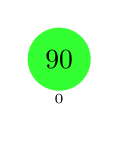
\begin{tikzpicture}[level distance=15mm, sibling distance=20mm]
        \tikzstyle{every node}=[circle,inner sep=1pt, minimum size=8mm]
        \tikzstyle{level 1}=[sibling distance=60mm]
        \tikzstyle{level 2}=[sibling distance=30mm]
        \tikzstyle{level 3}=[sibling distance=15mm]
        \tikzstyle{level 4}=[sibling distance=10mm]
        \node [fill=green!80] {90} node [below=3pt] {\tiny 0} ;
    \end{tikzpicture}
    \caption{Step 1}
\end{minipage}
\vspace{1cm}

\begin{minipage}{0.8\textwidth}
    \centering
    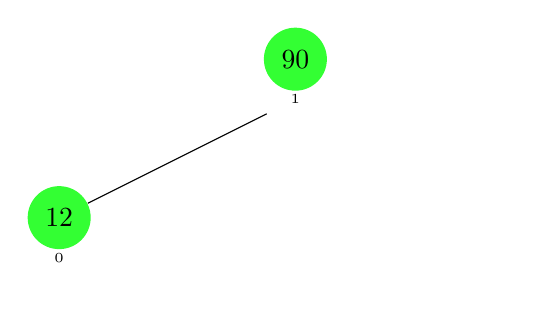
\begin{tikzpicture}[level distance=15mm, sibling distance=20mm]
        \tikzstyle{every node}=[circle,inner sep=1pt, minimum size=8mm]
        \tikzstyle{level 1}=[sibling distance=60mm]
        \tikzstyle{level 2}=[sibling distance=30mm]
        \tikzstyle{level 3}=[sibling distance=15mm]
        \tikzstyle{level 4}=[sibling distance=10mm]
        \node [fill=green!80] {90} node [below=3pt] {\tiny 1} child {node [fill=green!80] {12} node [below=3pt] {\tiny 0} } child[fill=none] {edge from parent[draw=none]};
    \end{tikzpicture}
    \caption{Step 2}
\end{minipage}
\vspace{1cm}

\begin{minipage}{0.8\textwidth}
    \centering
    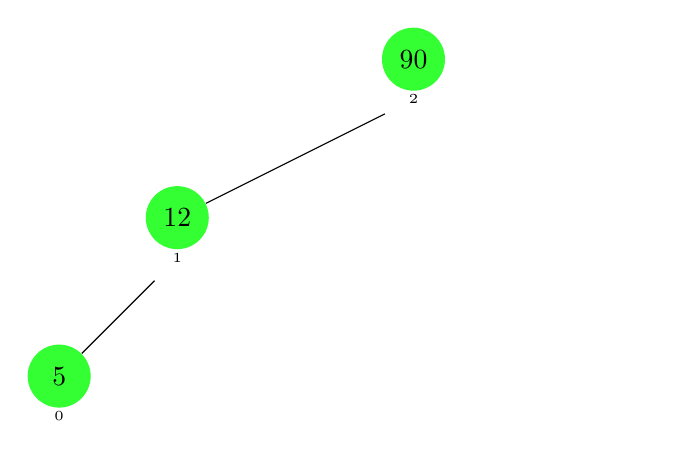
\begin{tikzpicture}[level distance=15mm, sibling distance=20mm]
        \tikzstyle{every node}=[circle,inner sep=1pt, minimum size=8mm]
        \tikzstyle{level 1}=[sibling distance=60mm]
        \tikzstyle{level 2}=[sibling distance=30mm]
        \tikzstyle{level 3}=[sibling distance=15mm]
        \tikzstyle{level 4}=[sibling distance=10mm]
        \node [fill=green!80] {90} node [below=3pt] {\tiny 2} child {node [fill=green!80] {12} node [below=3pt] {\tiny 1} child {node [fill=green!80] {5} node [below=3pt] {\tiny 0} } child[fill=none] {edge from parent[draw=none]}} child[fill=none] {edge from parent[draw=none]};
    \end{tikzpicture}
    \caption{Step 3}
\end{minipage}
\vspace{1cm}

\end{figure}
\newpage

\begin{figure}[h!]
\centering

\begin{minipage}{0.8\textwidth}
    \centering
    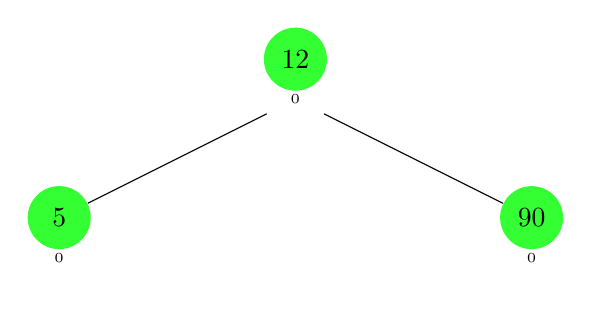
\begin{tikzpicture}[level distance=15mm, sibling distance=20mm]
        \tikzstyle{every node}=[circle,inner sep=1pt, minimum size=8mm]
        \tikzstyle{level 1}=[sibling distance=60mm]
        \tikzstyle{level 2}=[sibling distance=30mm]
        \tikzstyle{level 3}=[sibling distance=15mm]
        \tikzstyle{level 4}=[sibling distance=10mm]
        \node [fill=green!80] {12} node [below=3pt] {\tiny 0} child {node [fill=green!80] {5} node [below=3pt] {\tiny 0} } child {node [fill=green!80] {90} node [below=3pt] {\tiny 0} };
    \end{tikzpicture}
    \caption{Step 4}
\end{minipage}
\vspace{1cm}

\begin{minipage}{0.8\textwidth}
    \centering
    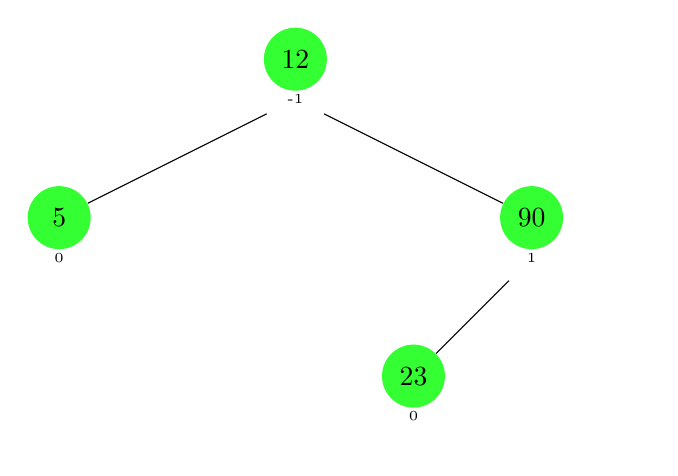
\begin{tikzpicture}[level distance=15mm, sibling distance=20mm]
        \tikzstyle{every node}=[circle,inner sep=1pt, minimum size=8mm]
        \tikzstyle{level 1}=[sibling distance=60mm]
        \tikzstyle{level 2}=[sibling distance=30mm]
        \tikzstyle{level 3}=[sibling distance=15mm]
        \tikzstyle{level 4}=[sibling distance=10mm]
        \node [fill=green!80] {12} node [below=3pt] {\tiny -1} child {node [fill=green!80] {5} node [below=3pt] {\tiny 0} } child {node [fill=green!80] {90} node [below=3pt] {\tiny 1} child {node [fill=green!80] {23} node [below=3pt] {\tiny 0} } child[fill=none] {edge from parent[draw=none]}};
    \end{tikzpicture}
    \caption{Step 5}
\end{minipage}
\vspace{1cm}

\end{figure}
\newpage

\end{document}
